% lintrans - The linear transformation visualizer
% Copyright (C) 2021-2022 D. Dyson (DoctorDalek1963)

% This program is licensed under GNU GPLv3, available here:
% <https://www.gnu.org/licenses/gpl-3.0.html>

\documentclass[../main.tex]{subfiles}

\begin{document}

Please note, throughout this section, every code snippet will have two comments at the top. The first is the git commit hash that the snippet was taken from\footnote{A history of all commits can be found in the GitHub repository\cite{lintrans-github}}. The second comment is the file name. The line numbers of the snippet reflect the line numbers of the file from where the snippet was taken. After a certain point, I introduced copyright comments at the top of every file. These are always omitted here.

\subsection{Matrices backend\label{development:matrices-backend}}

\subsubsection{\texttt{MatrixWrapper} class\label{development:matrices-backend:MatrixWrapper-class}}

The first real part of development was creating the \texttt{MatrixWrapper} class. It needs a simple instance dictionary to be created in the constructor, and it needs a way of accessing the matrices. I decided to use Python's \texttt{\_\_getitem\_\_()} and \texttt{\_\_setitem\_\_()} special methods\cite{python-3-special-methods} to allow indexing into a \texttt{MatrixWrapper} object like \texttt{wrapper['M']}. This simplifies using the class.

%: 29ec1fedbf307e3b7ca731c4a381535fec899b0b
%: src/lintrans/matrices/wrapper.py

This code is very simple. The constructor (\texttt{\_\_init\_\_()}) creates a dictionary of matrices which all start out as having no value, except the identity matrix \textbf{I}. The \texttt{\_\_getitem\_\_()} and \texttt{\_\_setitem\_\_()} methods allow the user to easily get and set matrices just like a dictionary, and \texttt{\_\_setitem\_\_()} will raise an error if the name is invalid. This is a very early prototype, so it doesn't validate the type of whatever the user is trying to assign it to yet. This validation will come later.

I could make this class subclass \texttt{dict}, since it's basically just a dictionary at this point, but I want to extend it with much more functionality later, so I chose to handle the dictionary stuff myself.

I then had to write unit tests for this class, and I chose to do all my unit tests using a framework called \texttt{pytest}.

%: 29ec1fedbf307e3b7ca731c4a381535fec899b0b
%: tests/test_matrix_wrapper.py

These tests are quite simple and just ensure that the expected behaviour works the way it should, and that the correct errors are raised when they should be. It verifies that matrices can be assigned, that every valid name works, and that the identity matrix \textbf{I} cannot be assigned to.

The function decorated with \mintinline{python}{@pytest.fixture} allows functions to use a parameter called \texttt{wrapper} and \texttt{pytest} will automatically call this function and pass it as that parameter. It just saves on code repetition.

\subsubsection{Rudimentary parsing and evaluating\label{development:matrices-backend:rudimentary-parsing-and-evaluating}}

This first thing I did here was improve the \texttt{\_\_setitem\_\_()} and \texttt{\_\_getitem\_\_()} methods to validate input and easily get transposes and simple rotation matrices.

%: f89fc9fd8d5917d07557fc50df3331123b55ad6b
%: src/lintrans/matrices/wrapper.py:60-81

In this method, I'm now casting all the values to floats. This is very simple validation, since this cast will raise \mintinline{python}{ValueError} if it fails to cast the value to a float. I should've declared \texttt{:raises ValueError:} in the docstring, but this was an oversight at the time.

%: f89fc9fd8d5917d07557fc50df3331123b55ad6b
%: src/lintrans/matrices/wrapper.py:27-59

This \texttt{\_\_getitem\_\_()} method now allows for easily accessing transposes and rotation matrices by checking input with regular expressions. This makes getting matrices easier and thus makes evaluating full expressions simpler.

The \texttt{create\_rotation\_matrix()} method is also defined in this file and just uses the $\begin{psmallmatrix}\cos\theta & -\sin\theta\\\sin\theta & \cos\theta\end{psmallmatrix}$ formula from before:

%: f89fc9fd8d5917d07557fc50df3331123b55ad6b
%: src/lintrans/matrices/wrapper.py:158-168

At this stage, I also implemented a simple parser and evaluator using regular expressions. It's not great and it's not very flexible, but it can evaluate simple expressions.

%: f89fc9fd8d5917d07557fc50df3331123b55ad6b
%: src/lintrans/matrices/wrapper.py:83-155

I think the comments in the code speak for themselves, but we basically split the expression up into groups to be added, and then for each group, we multiply every matrix in that group to get its value, and then add all these values together at the end.

This code is objectively bad. At the time of writing, it's now quite old, so I can say that. This code has no real error handling, and line 48 introduces the glaring error that \texttt{'A++B'} is now a valid expression because we disregard empty strings. Not to mention the fact that the method is called \texttt{parse\_expression()} but actually evaluates an expression. All these issues will be fixed in the future, but this was the first implementation of matrix evaluation, and it does the job decently well.

I then implemented several tests for this parsing.

%: 60e0c713b244e097bab8ee0f71142b709fde1a8b
%: tests/test_matrix_wrapper_parse_expression.py

These test lots of simple expressions, but don't test any more complicated expressions, nor do they test any validation, mostly because validation doesn't really exist at this point. \texttt{'A++B'} is still a valid expression and is equivalent to \texttt{'A+B'}.

\subsubsection{Simple matrix expression validation\label{development:matrices-backend:simple-matrix-expression-validation}}

My next major step was to implement proper parsing, but I procrastinated for a while and first implemented proper validation.

%: 39b918651f60bc72bc19d2018075b24a6fc3af17
%: src/lintrans/_parse/matrices.py:9-55

Here, I'm using a BNF schema to programmatically generate a regular expression. I use a function to generate this pattern and assign it to a variable when the module is initialized. This is because the pattern compilation is expensive and it's more efficient to compile the pattern once and then just use it in the \texttt{validate\_matrix\_expression()} function.

I also created a method \texttt{is\_valid\_expression()} in \texttt{MatrixWrapper}, which just validates a given expression. It uses the aforementioned \texttt{validate\_matrix\_expression()} and also checks that every matrix referenced in the expression is defined in the wrapper.

%: 39b918651f60bc72bc19d2018075b24a6fc3af17
%: src/lintrans/matrices/wrapper.py:99-117

I then implemented some simple tests to make sure the function works with valid and invalid expressions.

%: a0fb029f7da995803c24ee36e7e8078e5621f676
%: tests/_parse/test_parse_and_validate_expression.py

Here, we test some valid data, some definitely invalid data, and some edge cases. At this stage, \texttt{'A--1B'} was considered a valid expression. This was a quirk of the validator at the time, but I fixed it later. This should obviously be an invalid expression, especially since \texttt{'A--B'} is considered invalid, but \texttt{'A--1B'} is valid.

The \mintinline{python}{@pytest.mark.parametrize} decorator on line 35 means that \texttt{pytest} will run one test for valid inputs, and then another test for invalid inputs, and these will count as different tests. This makes it easier to see which tests failed and then debug the app.

\subsubsection{Parsing matrix expressions\label{development:matrices-backend:parsing-matrix-expressions}}

Parsing is quite an interesting problem and something I didn't feel able to tackle head-on, so I wrote the unit tests first. I had a basic idea of what I wanted the parser to return, but no real idea of how to implement that. My unit tests looked like this:

%: e9f7a81892278fe70684562052f330fb3a02bf9b
%: tests/_parse/test_parse_and_validate_expression.py:40-75

I just had example inputs and what I expected as output. I also wanted the parser to ignore whitespace. The decorator on line 33 just skips the test because the parser wasn't implemented yet.

When implementing the parser, I first had to tighten up validation to remove anomalies like \texttt{'A--1B'} being valid. I did this by factoring out the optional minus signs from being part of a number, to being optionally in front of a number. This eliminated this kind of repetition and made \texttt{'A--1B'} invalid, as it should be.

%: fd80d8d3b0e975e92dcc7c10f1f0f1276879f408
%: src/lintrans/_parse/matrices.py:32-45

The code can be a bit hard to read with all the RegEx stuff, but the BNF illustrates these changes nicely.

Compare the old version:

%: 39b918651f60bc72bc19d2018075b24a6fc3af17
%: src/lintrans/_parse/matrices.py:38-49 strip

to the new version:

%: fd80d8d3b0e975e92dcc7c10f1f0f1276879f408
%: src/lintrans/_parse/matrices.py:61-72 strip

Then once I'd fixed the validation, I could implement the parser itself.

%: fd80d8d3b0e975e92dcc7c10f1f0f1276879f408
%: src/lintrans/_parse/matrices.py:86-128

It works similarly to the old \texttt{MatrixWrapper.parse\_expression()} method in \S\ref{development:matrices-backend:rudimentary-parsing-and-evaluating} but with a powerful list comprehension at the end. It splits the expression up into groups and then uses some RegEx magic to find all the matrices in these groups as a tuple.

This method passes all the unit tests, as expected.

My next step was then to rewrite the evaluation to use this new parser, like so (method name and docstring removed):

%: a453774bcdf824676461f9b9b441d7b94969ea55
%: src/lintrans/matrices/wrapper.py:168-191

Here, we go through the list of tuples and evaluate the matrix represented by each tuple, putting this together in a list as we go. Then at the end, we simply reduce the sublists and then reduce these new matrices using a list comprehension in the \texttt{reduce()} call using \texttt{add} and \texttt{matmul} from the \texttt{operator} library. It's written in a functional programming style, and it passes all the previous tests.

\subsection{Initial GUI\label{development:initial-gui}}

\subsubsection{First basic GUI\label{development:initial-gui:first-basic-gui}}

The discrepancy in all the GUI code between \texttt{snake\_case} and \texttt{camelCase} is because Qt5 was originally a C++ framework that was adapted into PyQt5 for Python. All the Qt API is in \texttt{camelCase}, but my Python code is in \texttt{snake\_case}.

%: 93ce763f7b993439fc0da89fad39456d8cc4b52c
%: src/lintrans/gui/main_window.py

\fsbsl{development/93ce763f7b993439fc0da89fad39456d8cc4b52c/gui.png}{The first version of the GUI}{A lot of the methods here don't have implementations yet, but they will. This version is just a very early prototype to get a rough draft of the GUI.\par I create the widgets and layouts in the constructor as well as configuring all of them. The most important non-constructor method is \texttt{update\_render\_buttons()}. It gets called whenever the text in \texttt{text\_input\_expression} is changed. This happens because we connect it to the \texttt{textChanged} signal on line 35.\par The big white box here will eventually be replaced with an actual viewport. This is just a prototype.}

\subsubsection{Numerical definition dialog\label{development:initial-gui:numerical-definition-dialog}}

My next major addition was a dialog that would allow the user to define a matrix numerically.

%: cedbd3ed126a1183f197c27adf6dabb4e5d301c7
%: src/lintrans/gui/dialogs/define_new_matrix.py

\fsbsl{development/cedbd3ed126a1183f197c27adf6dabb4e5d301c7/define-numerically-dialog.png}{The first version of the numerical definition dialog}{When I add more definition dialogs, I will factor out a superclass, but this is just a prototype to make sure it all works as intended.\par Hopefully the methods are relatively self explanatory, but they're just utility methods to update the GUI when things are changed. We connect the \texttt{QLineEdit} widgets to the \texttt{update\_confirm\_button()} slot to make sure the confirm button is always up to date.}

The \texttt{confirm\_matrix()} method just updates the instance's matrix wrapper with the new matrix. We pass a reference to the \texttt{LintransMainWindow} instance's matrix wrapper when we open the dialog, so we're just updating the referenced object directly.

In the \texttt{LintransMainWindow} class, we're just connecting a lambda slot to the button so that it opens the dialog, as seen here:

%: cedbd3ed126a1183f197c27adf6dabb4e5d301c7
%: src/lintrans/gui/main_window.py:66-68 strip

\subsubsection{More definition dialogs\label{development:initial-gui:more-definition-dialogs}}

I then factored out the constructor into a \texttt{DefineDialog} superclass so that I could easily create other definition dialogs.

%: 5d04fb7233a03d0cd8fa0768f6387c6678da9df3
%: src/lintrans/gui/dialogs/define_new_matrix.py:22-60

This superclass just has a constructor that subclasses can use. When I added the \texttt{DefineAsARotationDialog} class, I also moved the cancel and confirm buttons into the constructor and added abstract methods that all dialog subclasses must implement.

%: 0d534c35c6a4451e317d41a0d2b3ecb17827b45f
%: src/lintrans/gui/dialogs/define_new_matrix.py:61-89

I then added the class for the rotation definition dialog.

%: 0d534c35c6a4451e317d41a0d2b3ecb17827b45f
%: src/lintrans/gui/dialogs/define_new_matrix.py:182-234

\fsbsr{development/0d534c35c6a4451e317d41a0d2b3ecb17827b45f/define-as-a-rotation-dialog.png}{The first version of the rotation definition dialog}{This dialog class just overrides the abstract methods of the superclass with its own implementations. This will be the pattern that all of the definition dialogs will follow.\par It has a checkbox for radians, since this is supported in \texttt{create\_rotation\_matrix()}, but the textbox only supports numbers, so the user would have to calculate some multiple of $\pi$ and paste in several decimal places. I expect people to only use degrees, because these are easier to use.}

I also then implemented a simple \texttt{DefineAsAnExpressionDialog}, which evaluates a given expression in the current \texttt{MatrixWrapper} context and assigns the result to the given matrix name.

%: d5f930e15c3c8798d4990486532da46e926a6cb9
%: src/lintrans/gui/dialogs/define_new_matrix.py:241-277

My next dialog that I wanted to implement was a visual definition dialog, which would allow the user to drag around the basis vectors to define a transformation. However, I would first need to create the \texttt{lintrans.gui.plots} package to allow for actually visualizing matrices and transformations.

\subsection{Visualizing matrices\label{development:visualizing-matrices}}

\subsubsection{Asking strangers on the internet for help\label{development:visualizing-matrices:asking-strangers-on-the-internet-for-help}}

After creating most of the GUI skeleton, I wanted to build the viewport. Unfortunately, I had no idea what I was doing.

While looking through the PyQt5 docs, I found a pretty comprehensive explanation of the Qt5 \enquote{Graphics View Framework}\cite{pyqt5-graphics-view-framework}, which seemed pretty good, but not really what I was looking for. I wanted a way to easily draw lots of straight, parallel lines. This framework seemed more focussed on manipulating objects on a canvas, almost like sprites. I knew of a different Python library called \texttt{matplotlib}, which has various backends available. I learned that it could be embedded in a standard PyQt5 GUI, so I started doing some research.

I didn't get very far with \texttt{matplotlib}. I hadn't used it much before and it's designed for visualizing data. It can draw manually defined straight lines on a canvas, but that's not what it's designed for and it's not very good at it. Thankfully, my horrific \texttt{matplotlib} code has been lost to time. I used the \texttt{Qt5Agg} backend from \texttt{matplotlib} to create a custom PyQt5 widget for the GUI and I could graph randomly generated data with it after following a tutorial\cite{matplotlib-pyqt5-tutorial}.

I realised that I wasn't going to get very far with \texttt{matplotlib}, but I didn't know what else to do. I couldn't find any relevant examples on the internet, so I decided to post a question on a forum myself. I'd had experience with StackOverflow and its unfriendly community before, so I decided to ask the \texttt{r/learnpython} subreddit\cite{reddit-framework-question}.

I only got one response, but it was incredibly helpful. The person told me that if I couldn't find an easy way to do what I wanted, I could write a custom PyQt5 widget. I knew this was possible with a class that just inherited from \texttt{QWidget}, but had no idea how to actually make something useful. Thankfully, this person provided a link to a GitLab repository of theirs, where they had multiple examples of custom widgets with PyQt5\cite{gitlab-custom-widgets}.

When looking through this repo, I found out how to draw on a widget like a simple canvas. All I have to do is override the \texttt{paintEvent()} method and use a \texttt{QPainter} object to draw on the widget. I used this knowledge to start creating the actual viewport for the GUI, starting with the background axes.

\subsubsection{Creating the plots package\label{development:visualizing-matrices:creating-the-plots-package}}

Initially, the \texttt{lintrans.gui.plots} package just has some classes for widgets. \texttt{TransformationPlotWidget} acts as a base class and then \texttt{ViewTransformationWidget} acts as a wrapper. I will expand this class in the future.

%: 4af63072b383dc9cef9adbb8900323aa007e7f26
%: src/lintrans/gui/plots/plot_widget.py

\fsbsl{development/4af63072b383dc9cef9adbb8900323aa007e7f26/gui.png}{The GUI with background axes}{The meat of this class is the \texttt{draw\_widget()} method. Right now, this method only draws the background axes. My next step is to implement basis vector attributes and draw them in \texttt{draw\_widget()}. After changing the the \texttt{plot} attribute in \texttt{LintransMainWindow} to an instance of \texttt{ViewTransformationWidget}, the plot was visible in the GUI.\par I then refactored the code slightly to rename \texttt{draw\_widget()} to \texttt{draw\_background()} and then call it from the \texttt{paintEvent()} method in \texttt{ViewTransformationWidget}.}

\subsubsection{Implementing basis vectors\label{development:visualizing-matrices:implementing-basis-vectors}}

My first step in implementing basis vectors was to add some utility methods to convert between coordinate systems. The matrices are using Cartesian coordinates with $(0, 0)$ in the middle, positive $x$ going to the right, and positive $y$ going up. However, Qt5 is using standard computer graphics coordinates, with $(0, 0)$ in the top left, positive $x$ going to the right, and positive $y$ going down. I needed a way to convert Cartesian \enquote{grid} coordinates to Qt5 \enquote{canvas} coordinates, so I wrote some little utility methods.

%: 1fa7e1c61d61cb6aeff773b9698541f82fee39ea
%: src/lintrans/gui/plots/plot_widget.py:45-60

Once I had a way to convert coordinates, I could add the basis vectors themselves. I did this by creating attributes for the points in the constructor and creating a \texttt{transform\_by\_matrix()} method to change these point attributes accordingly.

%: 37e7c208a33d7cbbc8e0bb6c94cd889e2918c605
%: src/lintrans/gui/plots/plot_widget.py:92-112

I also created a \texttt{draw\_transformed\_grid()} method which gets called in \texttt{paintEvent()}.

%: 37e7c208a33d7cbbc8e0bb6c94cd889e2918c605
%: src/lintrans/gui/plots/plot_widget.py:122-128

I then changed the \texttt{render\_expression()} method in \texttt{LintransMainWindow} to call this new \texttt{transform\_by\_matrix()} method.

%: 37e7c208a33d7cbbc8e0bb6c94cd889e2918c605
%: src/lintrans/gui/main_window.py:229-235

Testing this new code shows that it works well.

\begin{figure}[H]
	\centering
	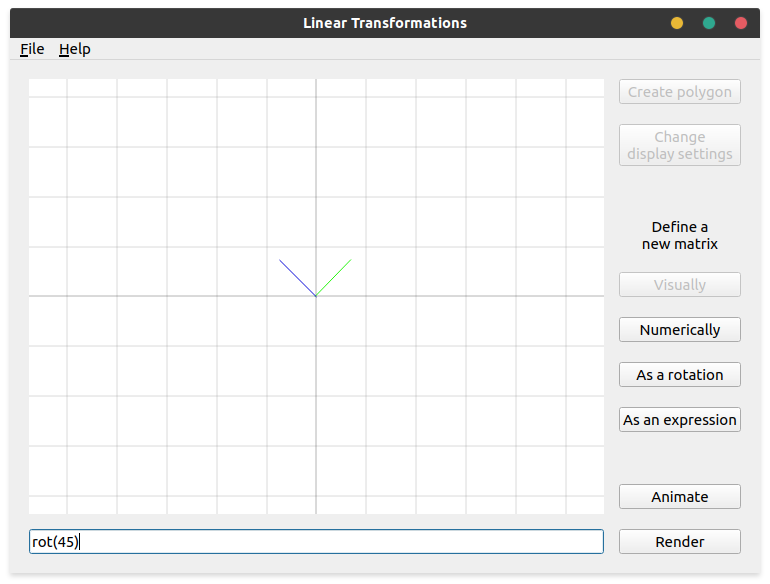
\includegraphics[width=0.7\linewidth]{development/37e7c208a33d7cbbc8e0bb6c94cd889e2918c605/gui.png}
	\caption{Basis vectors drawn for a $45\degree$ rotation}
	\label{fig:development:37e7c208a33d7cbbc8e0bb6c94cd889e2918c605:gui.png}
\end{figure}

\subsubsection{Drawing the transformed grid\label{development:visualizing-matrices:drawing-the-transformed-grid}}

After drawing the basis vectors, I wanted to draw the transformed version of the grid. I first created a \texttt{grid\_corner()} utility method to return the grid coordinates+ of the top right corner of the canvas. This allows me to find the bounding box in which to draw the grid lines.

%: 2ade98ac28d1c3f6691e4afa819142a3ab8e9fd9
%: src/lintrans/gui/plots/plot_widget.py:64-66

I then created a \texttt{draw\_parallel\_lines()} method that would fill the bounding box with a set of lines parallel to a given vector with spacing defined by the intersection with a given point.

%: 2ade98ac28d1c3f6691e4afa819142a3ab8e9fd9
%: src/lintrans/gui/plots/plot_widget.py:126-164

I then called this method from \texttt{draw\_transformed\_grid()}.

%: 2ade98ac28d1c3f6691e4afa819142a3ab8e9fd9
%: src/lintrans/gui/plots/plot_widget.py:166-178

\fsbsr{development/2ade98ac28d1c3f6691e4afa819142a3ab8e9fd9/gui.png}{Parallel lines being drawn for matrix $1.2\mathbf{I}$}{This worked quite well when the matrix involved no rotation, as seen in Figure~\ref{fig:development:2ade98ac28d1c3f6691e4afa819142a3ab8e9fd9:gui.png}, but this didn't work with rotation. When trying \texttt{rot(45)} for example, it looked the same as in Figure~\ref{fig:development:37e7c208a33d7cbbc8e0bb6c94cd889e2918c605:gui.png}.\par Also, the vectors aren't particularly clear. They'd be much better with arrowheads on their tips, but this is just a prototype. The arrowheads will come later.\par My next step was to make the transformed grid lines work with rotations.}

%: 7dfe1e24729562501e2fd88a839dca6b653a3375
%: src/lintrans/gui/plots/plot_widget.py:126-225 strip

This code checks if $x$ or $y$ is zero\footnote{We actually check if they're less than $10^{-12}$ to allow for floating point errors} and if they're not, then we have to use the standard straight line equation $y = mx + c$ to create parallel lines. We find our value of $m$ and then iterate through all the values of $c$ that keep the line within the bounding box.

\fsbsl{development/7dfe1e24729562501e2fd88a839dca6b653a3375/gui.png}{An example of a $20\degree$ rotation}{There are some serious logical errors in this code. It works fine for things like \texttt{3rot(45)} or \texttt{0.5rot(20)}, but something like \texttt{rot(115)} will leave the program hanging indefinitely.\par In fact, this code only works for rotations between $0\degree$ and $90\degree$, and will hang forever when given a matrix like $\begin{psmallmatrix}12 & 4 \\ -2 & 3\end{psmallmatrix}$, because it's just not very good.\par I will fix these issues in the future, but it works somewhat decently, so I decided to do animation next, because that sounded more fun.}

\subsubsection{Implementing animation\label{development:visualizing-matrices:implementing-animation}}

Now that I had a very crude renderer, I could create a method to animate a matrix. Eventually I want to be able to apply a given matrix to the currently rendered scene and animate between them. However, I wanted to start simple by animating from the identity to the given matrix.

%: 829a130af5aee9819bf0269c03ecfb20bec1a108
%: src/lintrans/gui/main_window.py:238-258

This code creates the \texttt{matrix\_move} variable and adds scaled versions of it to the identity matrix and renders that each frame. It's simple, but it works well for this simple use case. Unfortunately, it's very hard to show off an animation in a PDF, since all these images are static. The git commit hashes are included in the code snippets if you want to clone the repo\cite{lintrans-github}, checkout this commit, and run it yourself if you want.

\end{document}
